% -------------------------------------------------------------------------- %
% Style used is derived from the tufte-handout style available on GitHub at
% https://github.com/Tufte-LaTeX/tufte-latex
% License: Apache 2.0
\documentclass[nohyper, % Turn off defaults, customize hyperref locally
               ]{tufte-handout}

% -------------------------------------------------------------------------- %
% Define document-specific macros here
\DeclareRobustCommand{\ski}{\texttt{scikit-image}\xspace}
\DeclareRobustCommand{\spy}{SciPy\xspace} % Sadly, \sp is reserved (superscript)
\DeclareRobustCommand{\np}{NumPy\xspace}
% \newcommand{\release}{\pyc{import skimage;print(skimage.__version__)}\xspace}
\newcommand{\release}{0.11.3\xspace}
\newcommand{\eg}{e.g.\xspace}

% -------------------------------------------------------------------------- %
% Definitions used throughout the package
\title{\ski: the image processing toolkit for \spy}
\author[the \ski contributors]{the \ski contributors}
\date{6 July 2015} % Specify date, or comment out to use current date

% -------------------------------------------------------------------------- %
% Slightly tweak page layout so title fits on one line
\newgeometry{textwidth=27pc,      % 1pc wider than default
             marginparwidth=11pc, % 1pc narrower than default
             letterpaper,
             left=1in,
             top=1in,
             headsep=2\baselineskip,
             marginparsep=2pc,
             textheight=44\baselineskip,
             headheight=\baselineskip}

% Layout debugging
% \usepackage{showframe} % uncomment to debug page layout

% -------------------------------------------------------------------------- %
% Begin!
\begin{document}

\maketitle% tufte-handout command: prints title, author, and date

% Stay on brand
\begin{marginfigure}[-0.1cm]%
  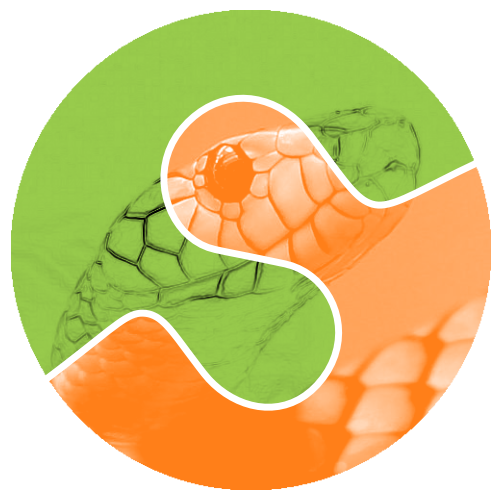
\includegraphics[width=\linewidth]{green_orange_snake.png}
  \label{fig:skimage_logo}
\end{marginfigure}

% Explain purpose
Welcome to \ski! This handout is designed to supplement and enhance the \ski tutorial materials, hosted on GitHub at \url{http://github.com/scikit-image/skimage-tutorials}. Our goal is to orient you to the package and provide you with a quick reference to common functions, so you can be as productive as possible!

\subsection{Where are my functions?} % (fold)
  \label{sec:Where_are_my_functions}
  Most of the functionality in \ski\marginnote[-0.1cm]{Unlike \textsc{matlab}, functions are grouped into \textit{subpackages} in \ski.} is located in \textit{subpackages}. This is similar to how \spy works. The reverse side of this handout has details about \ski subpackages available in version \release.
  % section Where_are_my_functions (end)

\subsection{Images are arrays} % (fold)
  \label{sub:images_are_arrays}

  \begin{marginfigure}[0.4cm]%
    \includegraphics[width=\linewidth]{tux_inset.png}
    \label{fig:tux_inset}
  \end{marginfigure}

  An image is simply a collection of data on a regular, two-dimensional grid. In \ski, we use \np arrays to represent images. Color images have more than one channel, \eg, red, green, and blue (RGB). Thus, the \np array for a color image is three-dimensional, with channel information in the final dimension.
  % subsection images_are_arrays (end)

\subsection{Talking our language} % (fold)
  \label{sub:talking_our_language}
  To avoid confusion, we refrain from using the terms \textit{x} or \textit{y}. Throughout the package, \ski refers to \textit{rows} (r) and \textit{columns} (c). When color data is present, \textit{channel} (ch) denotes the third dimension. \np arrays representing images are indexed via \pyv{arr[rows, columns]}.

  \begin{marginfigure}[-1.3cm]%
    \includegraphics[width=\linewidth]{row-col.png}
    \label{fig:row-col}
  \end{marginfigure}
  % subsection talking_our_language (end)

\subsection{Additional resources} % (fold)
  \label{sub:additional_resources}
  Please cite our paper\cite{van2014scikit} if you find \ski useful! The \ski website is located at \url{skimage.org/docs/stable}, including an API reference, user guide, and a gallery of examples. Issue tracking and development occur on GitHub at \url{github.com/scikit-image/scikit-image}. Please fork \ski\ -- your pull requests are appreciated!\\\medskip

  \noindent
  Interact with the community in our \texttt{gitter.im} chat room located at \url{gitter.im/scikit-image/scikit-image} or post on our Google Group at \url{groups.google.com/forum/#!forum/scikit-image}.
  % subsection additional_resources (end)

\newpage
\section{Road map to \ski} % (fold)
  \label{sec:road_map}
  Below are brief descriptions of each subpackage available in \ski \release, grouping features used for similar purposes.

  \begin{marginfigure}[1.9cm]%
    \includegraphics[width=\linewidth]{astronaut.png}
    \label{fig:astronaut}
  \end{marginfigure}

  \begin{description}
    \item[\pyv{skimage.color}] Color conversions.
    \begin{description}
      \item[\pyv{rgb2gray}] Convert a red-green-blue color image to grayscale.
      \item[\pyv{separate_stains}] Decompose color image into pathology stains.
    \end{description}
    \item[\pyv{skimage.data}] Test images.
    \begin{description}
      \item[\pyv{astronaut}] Image of the astronaut Eileen Collins\footnote[1][-0.3cm]{The \texttt{astronaut} test image. Please use this image in place of \texttt{lena}.}.
    \end{description}
    \item[\pyv{skimage.draw}] Drawing primitives such as lines or text.
    \item[\pyv{skimage.exposure}] Intensity and contrast adjustments.
    \item[\pyv{skimage.feature}] Feature detection and extraction.
    \item[\pyv{skimage.filters}] Whole-image changes like sharpening.
    \item[\pyv{skimage.future}] The bleeding edge, with potentially unstable API.
    \item[\pyv{skimage.graph}] Graph theory, shortest paths.
    \item[\pyv{skimage.io}] Read, save, and display images.
    \item[\pyv{skimage.measure}] Quantify image properties (length, shape).
    \item[\pyv{skimage.morphology}] Morphological operations like erosion and dilation.
    \item[\pyv{skimage.novice}] Simplified teaching interface.
    \item[\pyv{skimage.restoration}] Remove noise or deconvolve images.
    \item[\pyv{skimage.segmentation}] Partition an image into multiple regions.
    \item[\pyv{skimage.transform}] Warp or rotate images.
    \begin{description}
      \item[\pyv{radon/iradon}] The Radon transform and its inverse.
    \end{description}
    \item[\pyv{skimage.util}] Common public utility functions.
    \begin{description}
      \item[\pyv{random_noise}] Make an existing image noisy.
      \item[\pyv{pad/crop}] Fast array padding/cropping.
    \end{description}
    \item[\pyv{skimage.viewer}] QT-based interactive GUI.
  \end{description}
  % section road_map (end)

\newpage
% Bibliography
\bibliography{bibliography}
\bibliographystyle{plainnat}

\end{document}
